%%% ----- general packages and settings ----- %%%
\documentclass[a4paper, ngerman, bibliography=totoc]{scrreprt}  %%, listof=totoc
\usepackage[T1]{fontenc}
\usepackage[utf8]{inputenc}
\usepackage{lmodern}
\usepackage{babel}
\usepackage{microtype} % fixes line breaks

%%% ----- bibliography ----- %%%
\usepackage[babel, german=quotes]{csquotes}
\usepackage[backend=biber, style=alphabetic-verb]{biblatex}
\bibliography{literatur}
\DeclareFieldFormat[article]{title}{#1\isdot} % http://golatex.de/formatierung-des-literaturverzeichnisses-mit-biblatex-t3988.html

%%% ----- references (http://tex.stackexchange.com/a/83051) ----- %%%
\usepackage{varioref}
\usepackage{hyperref}
\usepackage{cleveref}
\crefname{lstlisting}{Quelltext}{Quelltext}

%%% ----- listings ----- %%%
\usepackage{color}
\usepackage{listings}
\renewcommand{\lstlistingname}{Quelltext}
\renewcommand*{\lstlistlistingname}{Quelltextverzeichnis}

\definecolor{strings}{rgb}{0.69, 0.196, 0.267}
\definecolor{comments}{rgb}{0.247, 0.518, 0.173}
\definecolor{keywords}{rgb}{0.114, 0.180, 0.992}
\definecolor{linenumbers}{rgb}{0.25, 0.25, 0.25}

\lstset{ %
  belowcaptionskip=1\baselineskip{},
  breaklines=true,
  captionpos=b,
  commentstyle=\color{comments},
  keywordstyle=\color{keywords}\bfseries,
  morecomment=[s][\color{comments}]{/**}{*/},
  numbers=left,
  numbersep=16pt,
  numberstyle=\tiny\color{linenumbers},
  stringstyle=\color{strings},
  tabsize=2
}

%%% ----- graphics ----- %%%
\usepackage{graphicx}

%%% ---------- Document Data ----------
\title{Docker als unterstützendes Werkzeug für Softwareentwickler}
\subtitle{Erstes Kapitel der Bachelorarbeit}
\author{Bernhard Mayr}
\date{Version 1.1}

\begin{document}
\maketitle
\addchap{Kurzfassung}
Softwareentwicklung in Zeiten von Node.js, ASP.NET Core und Microservices impliziert die Verwendung einer Menge an Werkzeugen.
Die Hauptaufgabe des Softwareentwicklers ist es allerdings, Software zu entwickeln und nicht den Großteil seiner Zeit mit dem Erlernen und der Konfiguration dieser Werkzeuge zu verbringen.

Mit Docker wurde eine Plattform zur Vereinfachung der Softwareentwicklung auf Basis von Containervirtualisierung geschaffen, deren Ziele eine möglichst einfache Verwendung und Plattformunabhängigkeit sind.
Anhand der Geschichte der Containervirtualisierung wird in dieser Arbeit ein Vergleich zu herkömmlichen Virtualisierungsmöglichkeiten gezogen sowie die Funktionsweise und notwendigen Systemvoraussetzungen für die Verwendung von Containern dargestellt.
Nach einer Übersicht über bestehende Werkzeuge des Konfigurationsmanagements wird für Softwareentwickler eine Einführung in die Verwendung von Docker zu Entwicklungszwecken gegeben, wobei besonders auf Best-Practices und Integrationsmöglichkeiten in den Entwicklungsprozess Wert gelegt wird.

Am Beispiel verschiedener Anwendungsfälle wird gezeigt, wie der Entwicklungsprozess mithilfe von Docker stabiler und einheitlicher gestaltet werden kann, um das erklärte Ziel, einen produktiveren und angenehmeren Workflow für Softwareentwickler, zu erreichen.

Aktuelle Entwicklungen wie Eclipse Che und Windows Container zeigen, dass Containervirtualisierung im Allgemeinen und Docker im Speziellen eine große Zukunft bevorsteht.

\addchap{Abstract}

\tableofcontents
\chapter{Einleitung}
\section{Motivation}
Die tägliche Arbeit eines Softwareentwicklers beinhaltet die Verwendung von zahlreichen Werkzeugen.
Besonders bei der Entwicklung auf unterschiedlichen Plattformen führt die Kombination der zahlreichen Build-Tools, Compiler, Transpiler, Task-Runner, Paketmanager und Datenbanken schnell zu einer umfangreichen Kombination an Kommandos.
Projekte entwickeln sich weiter und neue Technologien erscheinen, schnell wird aus einem \texttt{npm run dev} ein \texttt{npm start} oder \texttt{mvn build} bricht aufgrund einer falschen Java-Version ab.
Die große Vielfalt der Werkzeuge, besonders im Web-Bereich, verlangt vom Entwickler, dass er sich für jedes Projekt das Wissen für ein neues Werkzeugset aneignet und dieses auch zu verwenden weiß.

Seit 2014 verspricht Docker mit dem Werbespruch \emph{"`Build, Ship, Run"'} eine Verbesserung des Softwareentwicklungsprozesses mithilfe von Containervirtualisierung.
Welche Möglichkeiten der Automatisierung für den Softwareentwickler gegeben sind, inwieweit ein plattformunabhängiger Entwicklungsprozess möglich ist und ob sich durch den Einsatz von Docker die Lernkurve eines Entwicklers beim Einstieg in ein Softwareprojekt verringern lässt, sind motivierende Gründe für diese Bachelorarbeit.

\section{Ziel}
Durch exemplarisches Lösen typischer Probleme, mit denen Softwareentwickler häufig konfrontiert sind, soll dem Leser die Verwendung und Flexibilität von Docker gezeigt werden.
Weiters sollen Softwareentwickler automatisierbare Probleme erkennen und verstehen, ob und wie Docker in diesen Fällen zu einer zeit- und ressourcensparenden Lösung beitragen könnte.

Zur Verdeutlichung dieser entwicklergesteuerten Sicht auf Docker werden in der Arbeit verschiedene Virtualisierungstechniken verglichen und in der Funktionsweise und dem Einsatzzweck von Docker abgegrenzt.
Die grundlegenden, für den Entwickler notwendigen Konzepte von Docker werden ebenso geschildert wie eine Übersicht und Erklärung der in Verbindung mit Docker am häufigsten eingesetzten Werkzeuge.

% \section{Glossar}
% \begin{description}
%    \item[Vollvirtualisierung]
%    \item [DevOps]
% \end{description}

\chapter{Virtualisierung}
\label{cha:virtualisierung}
\section{Beweggründe und Geschichte}
\label{sec:virtualisierungsgeschichte}
- IBM als Beginn der Virtualisierung (kurze Erklärung der Geschichte)
- Warum wird heutzutage virtualisiert (Cloud-Umgebungen, Skalierung, Ressourcenverteilung) + Gartner-Trends
- Vorteile von Virtualisierung
- Nachteile von Virtualisierung
\section{Betriebssystemvirtualisierung}
\label{sec:betriebssystemvirtualisierung}
- Abgrenzung zu Hardwarevirtualisierung + Warum sinnvoll?
- kurz das Rechtekonzept mit den Ringen erklären
- Vor- & Nachteile bei Betriebssystemvirtualisierung
  - Speicherplatz
  - ganzes System kann, aber muss abstrahiert werden (Kernel, ...) 
\section{Containervirtualisierung}
\label{sec:containervirtualisierung}
- Produkte
- Grafik der Containervirtualisierung, Shared Host with mapped Syscalls
- Abschottung/Security
\subsection{Open Container Initiative (\emph{OCI})
\label{sec:open-container-initiative}
\subsection{Orchestrierungsmechanismen}
\label{sec:orchestrierungsmechanismen}
- DC/OS
- Mesosphere
- Swarm
- Kubernetes

\chapter{Konfigurationsmanagement}
\label{cha:konfigurationsmanagement}
Im Zusammenhang mit Docker und dem Softwareentwicklungsprozess werden oftmals zahlreiche weitere Werkzeuge genannt, die ähnliche Einsatzgebiete haben, oder in Kombination mit Docker den Prozess erheblich verbessern können.
In den folgenden Abschnitten werden die bekanntesten und am weitest verbreiteten Werkzeuge und deren jeweilige Einsatzzwecke vorgestellt.
Zusätzlich werden exemplarische Szenarien und die mögliche Kombination mit Docker aufgezeigt.

Die vorgestellten Werkzeuge dienen der Konfiguration der Entwicklungs- und Produktionsumgebung.
Wie~\autocite[29\psq]{Wolff201604} beschreibt, ließen sich diese Konfigurationen auch manuell vornehmen, doch damit treten erhebliche Probleme im Sinne der Testbarkeit, Reproduzierbarkeit und Automatisierung auf.
Ein noch größeres Problem stellt das implizite Wissen der Entwickler dar, das bei einer händischen Konfiguration nur verbal weitergegeben wird.
Auch dokumentierte Handbücher sind problematisch hinsichtlich der fehlerlosen Reproduzierbarkeit, da der Mensch im Gegensatz zum Computer dazu tendiert, fest definierte Abfolgen, trotz deren Spezifikation nicht fehlerlos durchzuführen, weshalb die Idee der Infrastrukturverwaltung in Versionskontrollsystemen entstanden ist.


\section{Infrastructure as Code}
\label{sec:infrastructureascode}
Da jede Anwendung eine Umgebung zur Ausführung benötigt und gerade in den letzten Jahren die Komplexität der Anwendungen im Hinblick auf die Anzahl und das Zusammenspiel zahlreicher Komponenten stark zugenommen hat, gibt es den Ansatz des \emph{Infrastructure as Code}.
Dabei werden wie zuvor bereits beschrieben, die Vorteile von Versionskontrollsystemen auf die Infrastruktur einer Anwendung angewandt.
Die Anwendungsinfrasktruktur wird nicht mehr händisch aufgebaut, sondern in Quelltexten abgelegt, wodurch das tatsächliche Erstellen der Infrastruktur auf diverse Werkzeuge verteilt wird.

Dadurch können wie in~\autocite[64\psqq]{Wolff201604} beschrieben, zahlreiche Vorteile erreicht werden.
\begin{itemize}
    \item Das System wird reproduzierbar, da manuelle Konfigurationsfehler vermieden werden.
    \item Bei einer konsequenten Durchführung entstehen idente Test- und Produktionsumgebungen, die sich bis zur Netzwerkebene nicht unterscheiden.
    \item Inkonsistente Systeme müssen nicht zwangsläufig repariert werden, wodurch sich Änderungen oder weitere Probleme ergeben können, sondern können entsorgt und sofort wieder aufgebaut werden.
    \item Die Infrastruktur ist nun reviewfähig, wordurch Probleme frühzeitig entdeckt werden.
    \item Wenn zusätzlich zu Infrastructure as Code auch noch verstärkt mit Virtualisierungstechniken gearbeitet wird, lässt sich zu Zeiten mit sehr hoher Last aufgrund der replizierbaren Umgebung einfach skalieren.
    \item Eine Dokumentation der gesamten Infrastruktur entsteht automatisch. Allerdings ohne, dass sie aktualisiert werden muss, denn der Infrastruktur-Quelltext ist die Dokumentation selbst zugleich.
    \item Durch diese Selbstdokumentation wird auch gewährleistet, dass an jede Softwareversion auch die dazu benötigte Infrastrukturversion gebunden wird. Diese Tatsache vereinfacht das Testen und das Ausrollen der Software um ein Vielfaches, da die Anforderungen an die Umgebung bekannt sind. Voraussetzung dafür ist allerdings, dass sich der Anwendungs- und Infrastrukturquelltext in einem gemeinsamen oder zumindest verknüften Repository der Versionsverwaltung befinden.
\end{itemize}
Damit dieses System funktioniert, dürfen Änderungen an der Infrastruktur \emph{allerdings nur} an den Konfigurationsdateien geändert werden. Da die Infrastruktur auf Basis dieser Konfiguration erstellt wird, gibt es keinen Datenrückfluss aus den Systemen in die Konfiguration.


\section{Werkzeuge}
\label{sec:konfigurationswerkzeuge}
\subsection{Vagrant}
\label{sub:vagrant}
Die folgenden Informationen und Quelltext-Beispiele sind aus \autocite{Vagrant:online} entnommen.
Vagrant ist ein Verwaltungswerkzeug für virtuelle Maschinen (siehe~\vref{sec:betriebssystemvirtualisierung}).
Die Idee von Vagrant ist, bestehende Virtualisierungslösungen wie VMware, VirtualBox oder AWS zu verwenden und darauf mit Werkzeugen die sich um die Bereitstellung von Software kümmern (vgl. \cref{sub:chef} oder \cref{sub:puppet}) fertige virtuelle Maschinen für Entwickler, Designer oder Infrastrukturmanager zu erstellen.
Aufgrund dieses Aufbaus können virtuelle Maschinen sehr einfach erweitert und daher generisch verwendet werden.
Um nicht immer jede virtuelle Maschine komplett neu erstellen zu müssen, gibt es bereits vorgefertigte \emph{Boxen}, die als Basis verwendet werden können.

Vagrant verwendet dazu eine eigene auf Ruby basierende DSL, die in den sogenannten Vagrantfiles Einsatz findet.
Diese Datei wird mit dem Quelltext mitversioniert und bietet den Entwicklern reproduzierbare, portable und plattformunabhängige Entwicklungsgeräte.
Das Konzept der Vagrantfiles ist auch in Docker (siehe~\vref{sec:dockerfiles}) wiederzufinden.
Dadurch verliert der bekannte Satz \emph{''But it works on my machine.''} stark an Bedeutung und Relevanz.
Anwendungen, die in der von Vagrant zur Vefügung gestellten Umgebung laufen, laufen auch immer in einer identen Umgebung, die sehr einfach mit Vagrant zur Verfügung gestellt werden können.

\subsubsection{Beispiel eines Apache Webservers mit Vagrant}
Mit den folgenden zwei Quelltextfragmenten wird ein Apache Webserver in einer virtuellen Maschine gestartet.
Das erste Skript ist ein ausführbares Shell-Skript, welches den Apache-Webserver installiert und vom Vagrantfile verwendet wird.
\lstinputlisting[caption=bootstrap.sh, language=bash]{listings/bootstrap.sh}
\label{lst:vagrant-bootstrap}
Der Vagrantfile beschreibt, dass die Box mit dem Namen \emph{hashicorp/precise64} verwendet wird und zum Erstellen der fertigen virtuellen Maschine ein Shell-Skript namens \emph{bootstrap.sh} ausgeführt werden soll.
\lstinputlisting[caption=Vagrantfile, language=Ruby]{listings/Vagrantfile}
\label{lst:vagrantfile}

Vagrant dient also zum Verwalten von virtuellen Maschinen, im besonderen und standardmäßigen Einsatzzweck, dem Verwalten von virtuellen Maschinen für Entwickler, die die Produktionsumgebung spiegeln und ein plattformunabhängiges Entwickeln ermöglichen.
Ein besonders nützlicher Anwendungsfall für Vagrant-Boxen sind Legacy-Systeme, für die eine vorkonfigurierte Entwicklungsumgebung benötigt wird, die allerdings auf keinem aktuellen Entwicklerrechner mehr verwendet wird.
So kann für einfache Bug-Fixes eine Vagrant-Entwicklerbox gestartet werden, ohne dass am Entwicklerrechner nicht mehr benötigte Werkzeuge installiert sein müssen.


\subsection{Chef}
\label{sub:chef}
Wie auf der offiziellen Homepage \autocite{Chef:online} von Chef beschrieben, ist Chef ein Werkzeug zur Infrastrukturautomatisierung. Daher konkurriert Chef mit den nächsten drei beschriebenen Werkzeugen, indem sie versuchen, dasselbe Problem zu lösen.

\autocite[34\psqq]{Wolff201604} liefert eine sehr gute und prägnante Einführung in das Werkzeug Chef.
Im Gegensatz zu einer Sammlung von Shell-Skripten, liefert Chef keinen Ablaufplan für das Erstellen eines Systems, sondern erstellt auf Basis gewisser Anforderungen Anweisungen, die das System in den Endzustand konfigurieren.
Dies hat den Vorteil, dass Sonderfälle minimiert werden, zum Beispiel ein schon vorhandenes veraltetes System muss nicht komplett entfernt und neuinstalliert werden, sondern kann durch das Aktualisieren der Anforderungen auf den neuen aktuellen Zustand gebracht werden.
Da das System auch nach mehrmaligem Ausführen gleich aussieht, spricht man von einer idempodenten Installationsprozedur.

Chef verwendet ebenso wie Vagrant eine Ruby-DSL, die in den sogenannten Rezepten (Recipes) Verwendung findet.
Diese Rezepte definieren die Anforderungen an die einzelnen Teile der Infrastruktur. Darin werden Konfigurationsdateien, Benutzer, Anwendungen, Plug-Ins und weitere Abhängigkeiten spezifiziert.
Da diese Rezepte mit steigender Komplexität des Systems an Übersichtlichkeit verlieren, gibt es die Gruppierung dieser in Kochbücher (Cookbooks).
Diese Kochbücher fassen mehrere Rezepte zusammen und bieten die Möglichkeit der Vorlagen (Templates) für Konfigurationsdateien, wodurch zahlreiche Server unterschiedlich parametrisiert werden können.
Chef kann entweder in einem Solo-Operationsmodus betrieben werden, oder als Chef-Zero für Testzwecke, oder in einer Client-Server-Umgebung, in der ein Chef-Server das Management der Konfigurationen übernimmt.
Von dort aus können mit geringem Aufwand neue Teile der Infrastruktur gestartet und bestehende gewartet werden. Dazu existieren als Erweiterung zu Chef Werkzeuge wie Knife\footnote{https://docs.chef.io/knife.html}.

\subsection{Puppet}
\label{sub:puppet}
Puppet wird noch etwas mehr, da ein Vergleich zu Chef gezogen wird, die restlichen Tools werden nur grob dargestellt, um deren Einsatzzweck zu dokumentieren.

\subsection{Ansible}
\label{sub:ansible}

\subsection{SaltStack}
\label{sub:saltstack}

\subsection{Packer}
\label{sub:packer}

\subsection{Habitat}
\label{sub:habitat}


\section{Kombinationsmöglichkeiten der Werkzeuge}
\label{sec:werkzeugkombinationsmoeglichkeiten}
\begin{figure}[htbp]
    \centering
    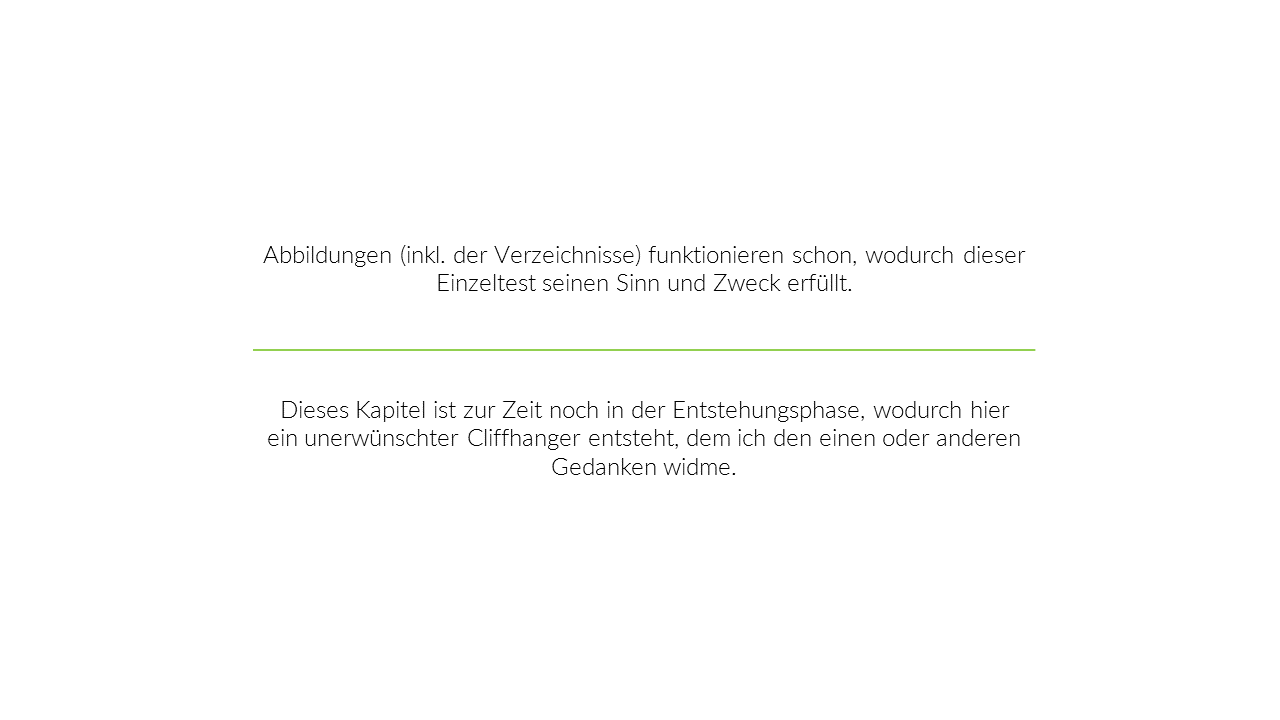
\includegraphics[width=0.9\linewidth,trim=190 160 190 160,clip]{images/cliffhanger}
    \caption{Das Zusammenspiel der Konfigurationsmanagementwerkzeuge}
\label{fig:konfigurationsmanagement-kombinationen}
\end{figure}

\chapter{Docker}
\label{cha:docker}
\section{Geschichte, Aufbau und Plattformen}
\label{sec:docker-basics}
\section{Komponenten des Docker-Systems}
\label{sec:docker-komponenten}
\section{Dockerfiles}
\label{sec:dockerfiles}
\section{Multi-Container-Anwendungen}
\label{sec:docker-multi-container-anwendungen}

\chapter{Szenarien für den Softwareentwicklungs-Workflow}
\label{cha:szenarien}
\section{Softwareevaluierung}
\label{sec:softwareevaluierung}
\section{Verbesserung des Build-Prozesses}
\label{sec:build-prozess-verbesserung}
\section{Testen mithilfe von Containern}
\label{sec:containerbasiertes-testen}
\section{Plattformübergreifende Übersetzung}
\label{sec:plattformuebergreifende-uebersetzung}
\section{IDE as a Container}
\label{sec:ideasacontainer}
\section{Replikation der Produktionsumgebung}
\label{sec:replikation-produktionsumgebung}

%%% --- TODO ---
%% Erkenntnisse
%% Resumee
%% - Zusammenfassung
%% - Ausblick
%%%

\addchap{Resümee}
\addsec{Zusammenfassung}

\addsec{Erkenntnisse}
Welche Vorteile Containervirtualisierung mit sich bringt. Nicht nur im Bereich der Servervirtualisierung, sondern auch für den Entwicklungsprozess.
Unglaubliche Anzahl an Tools, wobei nur wichtig ist, dass man weiß, dass es schon ein Tool für den Anwendungsfall gibt.

\addsec{Ausblick}
Der Leser dieser Arbeit hat nun gesehen welche Probleme sich mit Docker einfacher lösen lassen. Außerdem wurde ihm das Verständnis vermittelt, wie Docker funktioniert, weshalb der nächste Schritt der ist, sich selbst zu überlegen welche Anwendungsfälle mit Docker einfach umsetzbar sind.

Windows Container?

Bash on Windows on Linux

Standards, Reduzierung der Technologien

\listoffigures{}
\lstlistoflistings{}
\printbibliography{}
\end{document}
